\input{preambuloSimple.tex}
\title{	
	\normalfont \normalsize 
	\textsc{{\bf Ingeniería de Servidores (2016-2017)} \\ Grado en Ingeniería Informática \\ Universidad de Granada} \\ [25pt] % Your university, school and/or department name(s)
	\horrule{0.5pt} \\[0.4cm] % Thin top horizontal rule
	\huge Práctica 4. Benchmarks. \\ % The assignment title
	\horrule{2pt} \\[0.5cm] % Thick bottom horizontal rule
}

\author{Manuel Jiménez Molina} % Nombre y apellidos

\date{\normalsize\today} % Incluye la fecha actual

%----------------------------------------------------------------------------------------
% DOCUMENTO
%----------------------------------------------------------------------------------------

\begin{document}
	
	\maketitle % Muestra el Título
	
	\newpage %inserta un salto de página
	
	\tableofcontents % para generar el índice de contenidos
	
	\listoffigures
	
	\listoftables
	
	\newpage
	
	%NOTA: en caso de problema al compilar, compruebe que tiene el paquete: texlive-babel-spanish.noarch  \\
	
	
	
	
	\newpage
	
	%----------------------------------------------------------------------------------------
	%	Cuestión 1
	%----------------------------------------------------------------------------------------
	
	\section{Seleccione, instale y ejecute uno, comente los resultados.Atención: no es lo mismo un benchmark que una suite, instale un benchmark}
	
	
	Descargamos Phoronix de su página oficial\cite{ejercicio1-1}.\\
	
	Instalamos el paquete que descargado:\\
	\begin{center}
		sudo dpkg -i phoronix-test-suite\_6.8.0\_all.deb
	\end{center}
	A continuación ejecutamos phoronix con el comando:
	\begin{center}
		phoronix-test-suite
	\end{center}
	
	Nos muestra una lista de opciones a realizar, escogemos 'Run a test'. Veremos como nos muestra una lista de benchmarks a realizar:
	\begin{figure}[H] 
		\centering
		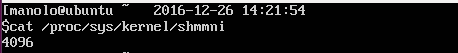
\includegraphics[scale=0.35]{ejercicio1-1.png} 
		\label{figura1} 
		\caption{Hacer un test con Phoronix}
	\end{figure} 
	
	Realizamos en benchmark número 65, llamado GpuTest. Vemos como se nos abre una pantalla en la que nos muestra con un entorno gráfico en 3D usando plot3d y OpenGL 3.0 nos muestra los fps (frames per seconds) y ms (delay o ping).Aquí vemos varias imágenes:
	
	\begin{figure}[H] 
		\centering
		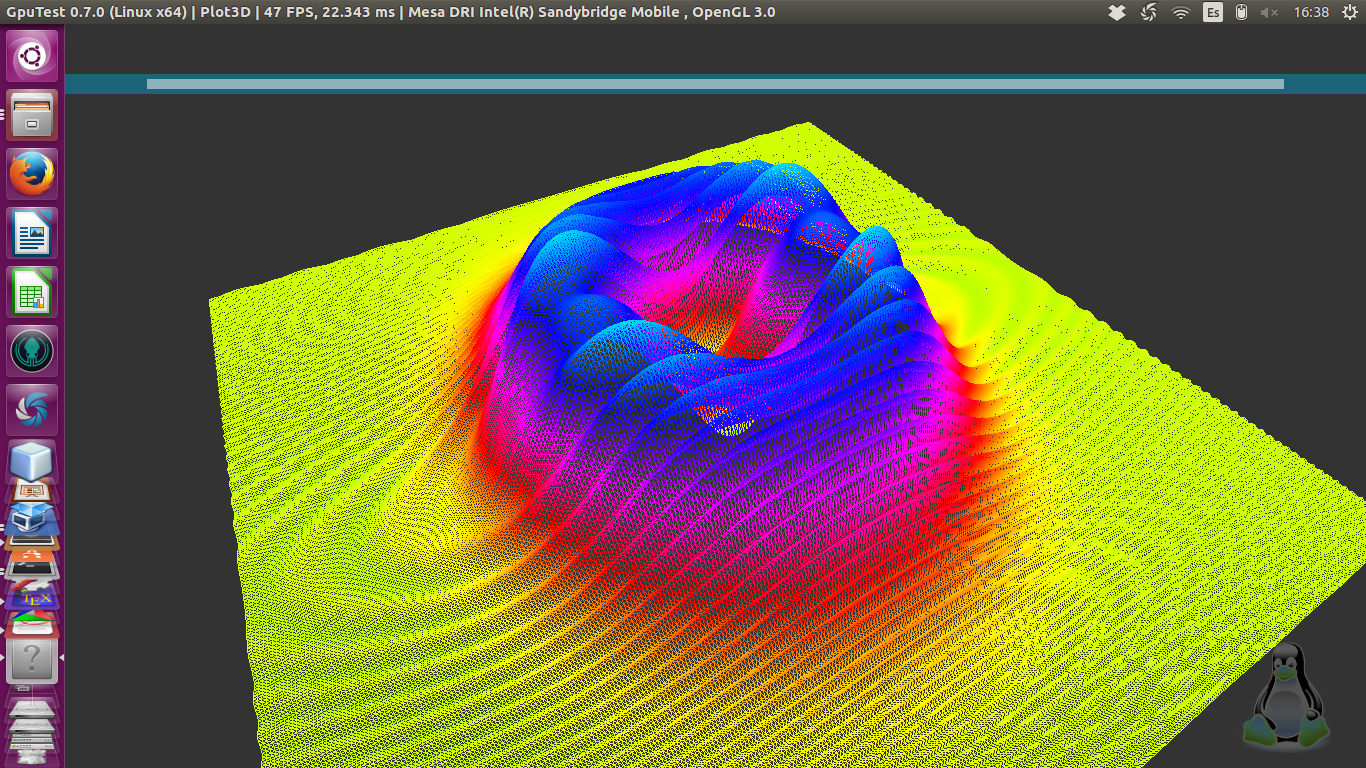
\includegraphics[scale=0.35]{ejercicio1-2.png} 
		\label{figura2} 
		\caption{Imagen 1: test de gpu en Phoronix}
	\end{figure}
	
	\begin{figure}[H] 
		\centering
		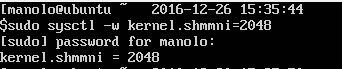
\includegraphics[scale=0.35]{ejercicio1-3.png} 
		\label{figura3} 
		\caption{Imagen 2: test de gpu en Phoronix}
	\end{figure}
	
	\begin{figure}[H] 
		\centering
		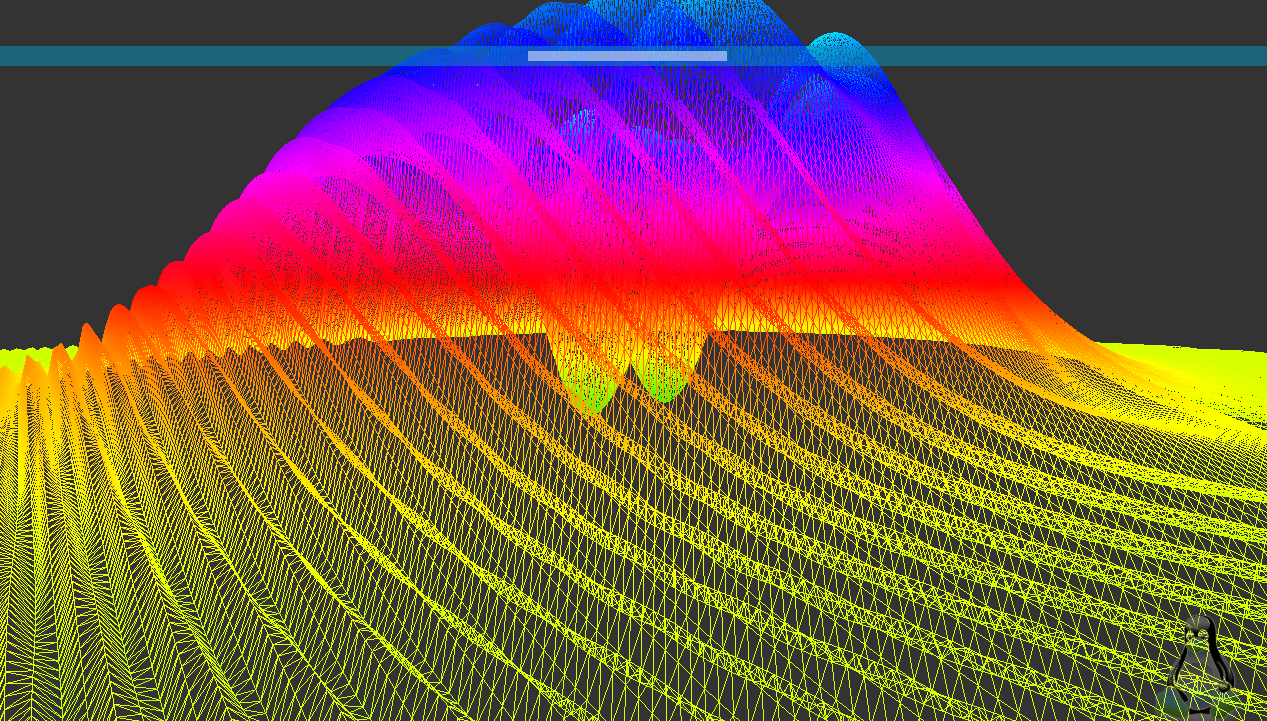
\includegraphics[scale=0.35]{ejercicio1-4.png} 
		\label{figura4} 
		\caption{Imagen 3: test de gpu en Phoronix}
	\end{figure}
	
    Podemos ver como nuestra gpu tiene entre 40-60 fps y su delay o ping son entorno a 20-30 segundos. Este test consiste en realizar 3 pruebas en modo ventana y otros 3 en modo pantalla completa, mostrando durante un tiempo determinado una gráfica para cada uno de ellos.\\
    Finalmente, nos muestra los resultados de los diferentes test, resaltando una media.
    
    \begin{figure}[H] 
    	\centering
    	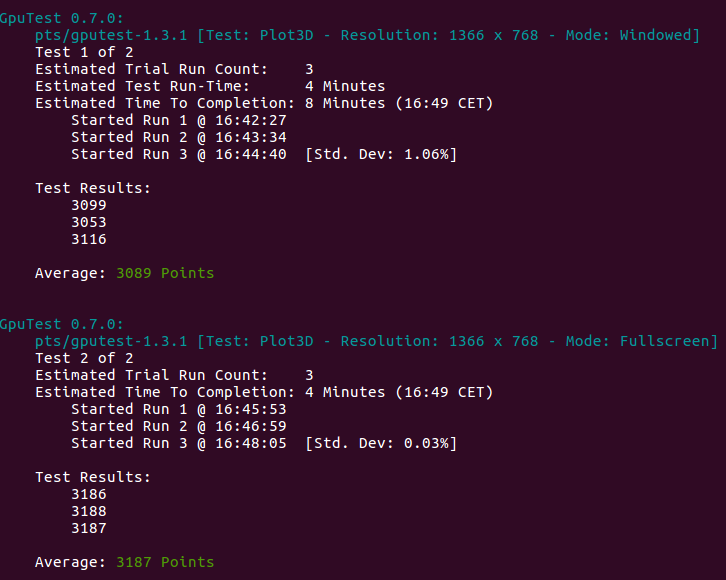
\includegraphics[scale=0.35]{ejercicio1-5.png} 
    	\label{figura5} 
    	\caption{Resultado test de gpu en Phoronix}
    \end{figure}
    
    Vemos como nos da una media para cada uno de los 3 test, con una puntuación de 3089 y 3187. Mirando las puntuaciones en esta página web\cite{ejercicio1-2} podemos ver por donde se encuentra nuestra gpu:
    
    \begin{figure}[H] 
    	\centering
    	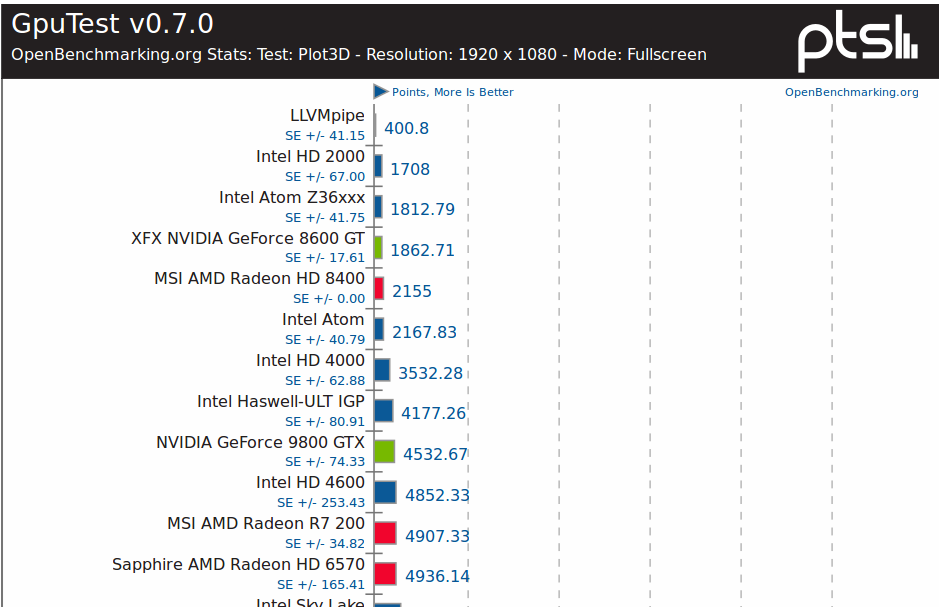
\includegraphics[scale=0.35]{ejercicio1-6.png} 
    	\label{figura6} 
    	\caption{Comparativas de benchmarks de gpu}
    \end{figure}
    
    Usando el comando lspci\cite{ejercicio1-3} podemos ver la lista de dispositivos PCI en nuestro equipo. De este modo vemos que tenemos una gráfica de Intel de segunda generación.
    
    
    \begin{figure}[H] 
    	\centering
    	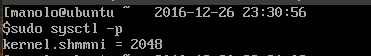
\includegraphics[scale=0.35]{ejercicio1-7.png} 
    	\label{figura7} 
    	\caption{Obtener gpu de nuestra máquina}
    \end{figure}
    
    Nuestra gráfica corresponde a un Intel HD Graphics 3000 o 2000\cite{ejercicio1-4}:
    \begin{figure}[H] 
     	\centering
     	
\includegraphics[scale=0.35]{ejercicio1-8.png} 
     	\label{figura8} 
     	\caption{Graficas 2ª generación de Intel}
     \end{figure}
     
     Viendo la comparativa de la imagen anterior y teniendo en cuenta la comparativa que nos ha hecho Phoronix dándonos una puntuación de entre 3089 y 3187, podemos decir que nuestra gráfica debe ser superior a Intel HD 2000 (puntuación de 1708) y menor que Intel HD 4000 (puntuación de 3532.28), por tanto seguramente nuestra gráfica sea una Intel HD 3000.
	%----------------------------------------------------------------------------------------
	%	Cuestión 2
	%----------------------------------------------------------------------------------------
	
	\section{De los parámetros que le podemos pasar al comando ¿Qué significa -c 5 ? ¿y -n 100? Monitorice la ejecución de ab contra alguna máquina (cualquiera) ¿cuántas “tareas” crea ab en el cliente?}
	
	Según el manual de apache benchmark (ab)\cite{ejercicio2-1} podemos saber que:
	\begin{itemize}
		\item -c 5: Opción para establecer el nivel de concurrencia, es decir, el número de solicitudes múltiples que se podrán realizar a la vez. Al ponerle 5 estaríamos realizando 5 peticiones a la vez.
		\item -n 100: Número de peticiones a realizar durante una sesión de benchmarking.
	\end{itemize}
	
	Vamos a realizar una monitorización para Apache que tenemos en Ubuntu Server con dirección 192.168.56.102 con concurrencia 5 y 100000 peticiones.A la vez que se ejecuta, monitorizamos los procesos que se crean en el cliente usando  ps\cite{ejercicio2-2} y wc\cite{ejercicio2-3}:
	
	
	\begin{figure}[H] 
	 	\centering
	 	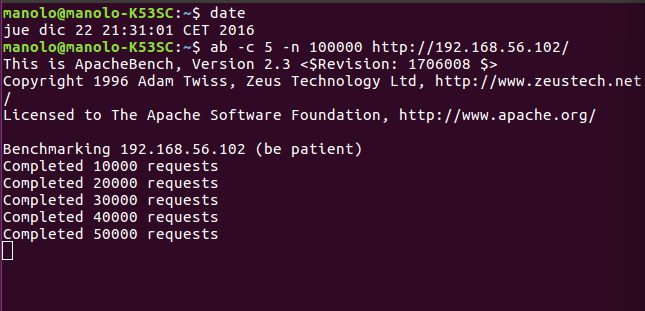
\includegraphics[scale=0.5]{ejercicio2-1.png} 
	 	\label{figura9} 
	 	\caption{Ejecutando ab en Apache Server}
	\end{figure}
	
	\begin{figure}[H] 
		\centering
		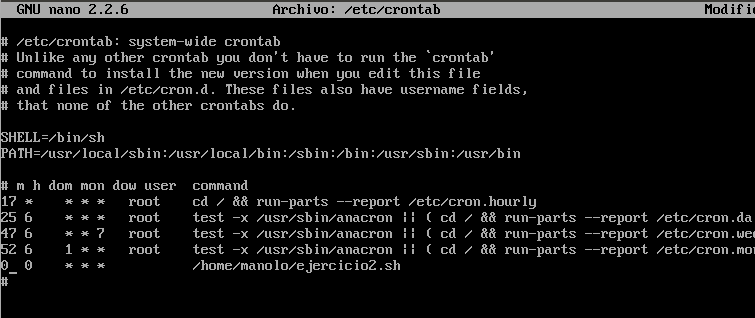
\includegraphics[scale=0.5]{ejercicio2-2.png} 
		\label{figura10} 
		\caption{Monitorizando ab en Apache Server con ps}
	\end{figure}
	
	Vemos como solo se crea un proceso en el cliente a pesar de haber indicado a apache benchmark concurrencia de 5.\\
	Aquí podemos ver como termina la ejecución de ab y observamos que indica que ha realizado la concurrencia que le indicamos.
	
	\begin{figure}[H] 
		\centering
		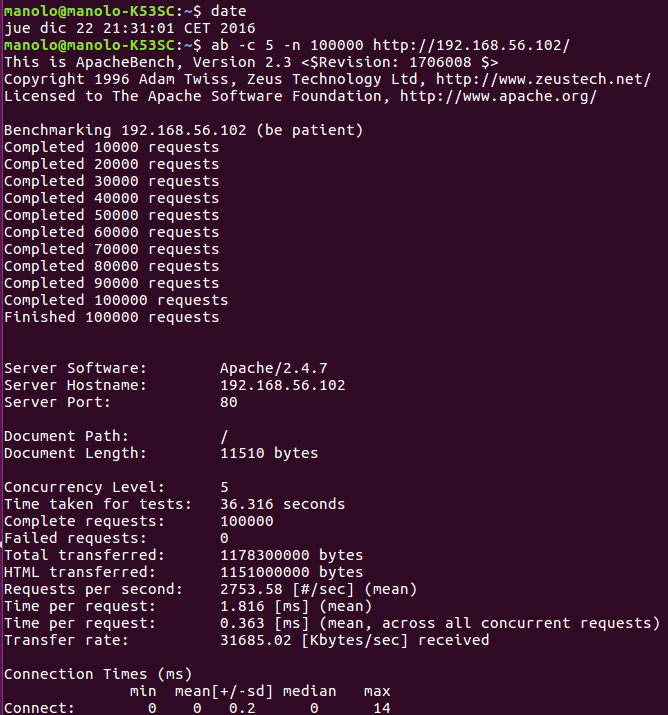
\includegraphics[scale=0.5]{ejercicio2-3.png} 
		\label{figura11} 
		\caption{Final de ejecución 1 de ab en Apache Server}
	\end{figure}
	
	\begin{figure}[H] 
		\centering
		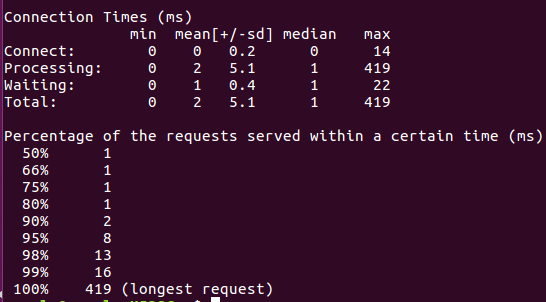
\includegraphics[scale=0.5]{ejercicio2-4.png} 
		\label{figura12} 
		\caption{Fin de ejecución 2 de ab en Apache Server}
	\end{figure}
	
	Esto quiere decir que ab crea concurrencia sin necesidad de crear más hebras.
	%----------------------------------------------------------------------------------------
	%	Cuestión 3
	%----------------------------------------------------------------------------------------
	
	\section{Ejecute ab contra a las tres máquinas virtuales (desde el SO anfitrión a las máquina virtuales de la red local) una a una (arrancadas por separado).¿Cuál es la que proporciona mejores resultados? Muestre y coméntelos. (Use como máquina de referencia Ubuntu Server para la comparativa)}
	
	Vamos a ejecutar ab desde la máquina anfitriona con concurrencia 5 y 1000 peticiones a las demás máquinas. Los resultados obtenidos son los siguientes:
	\begin{itemize}
		\item \textbf{Ubuntu Server}:
			\begin{figure}[H] 
				\centering
				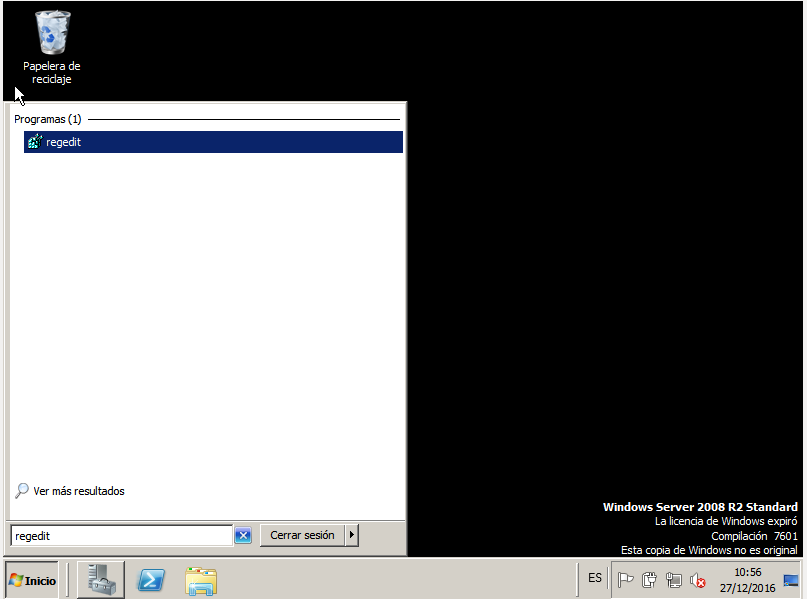
\includegraphics[scale=0.5]{ejercicio3-1.png} 
				\label{figura13} 
				\caption{Imagen 1: Resultados de ab para Ubuntu Server}
			\end{figure}
			
			\begin{figure}[H] 
				\centering
				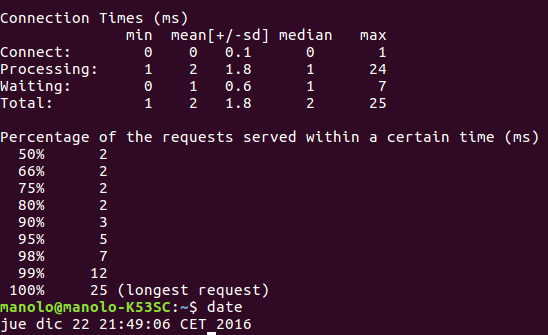
\includegraphics[scale=0.5]{ejercicio3-2.png} 
				\label{figura14} 
				\caption{Imagen 2: Resultados de ab para Ubuntu Server}
			\end{figure}
			
			Para Ubuntu Server podemos ver como el tiempo total del test es de 0.41 segundos. El tiempo media para cada petición es de 2.051 milisegundos. Dado que tenemos concurrencia 5, el tiempo medio de petición en concurrencia es de 2.051 ms / 5 = 0.410 ms.\\
			El total de bytes transferidos para Ubuntu Server es de 11783000 bytes.
		\item \textbf{Windows Server}:
			\begin{figure}[H] 
				\centering
				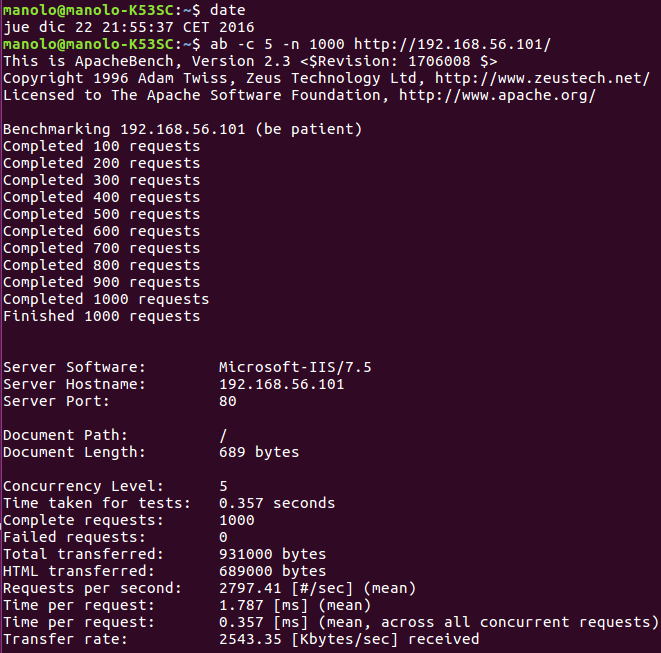
\includegraphics[scale=0.5]{ejercicio3-3.png} 
				\label{figura15} 
				\caption{Imagen 1: Resultados de ab para Windows Server}
			\end{figure}
			
			\begin{figure}[H] 
				\centering
				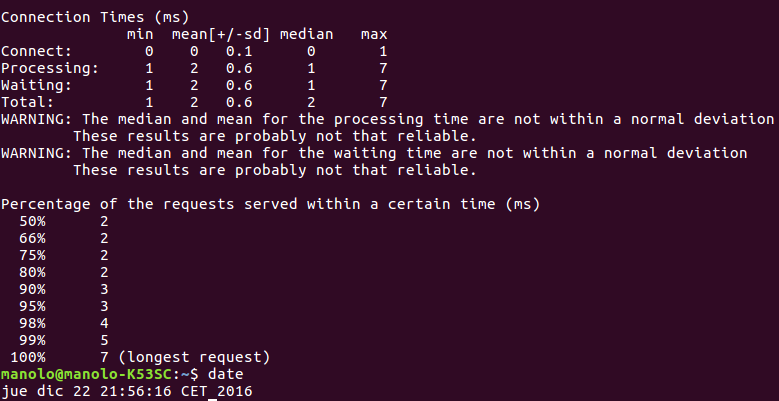
\includegraphics[scale=0.5]{ejercicio3-4.png} 
				\label{figura16} 
				\caption{Imagen 2: Resultados de ab para Windows Server}
			\end{figure}
			
			Para Windows Server podemos ver como el tiempo total del test es de 0.357 segundos. El tiempo media para cada petición es de 1.707 milisegundos. Dado que tenemos concurrencia 5, el tiempo medio de petición en concurrencia es de 1.707 ms / 5 = 0.357 ms.\\
			El total de bytes transferidos para Windows Server es de 931000 bytes.
			
		\item \textbf{CentOS}:
			\begin{figure}[H] 
				\centering
				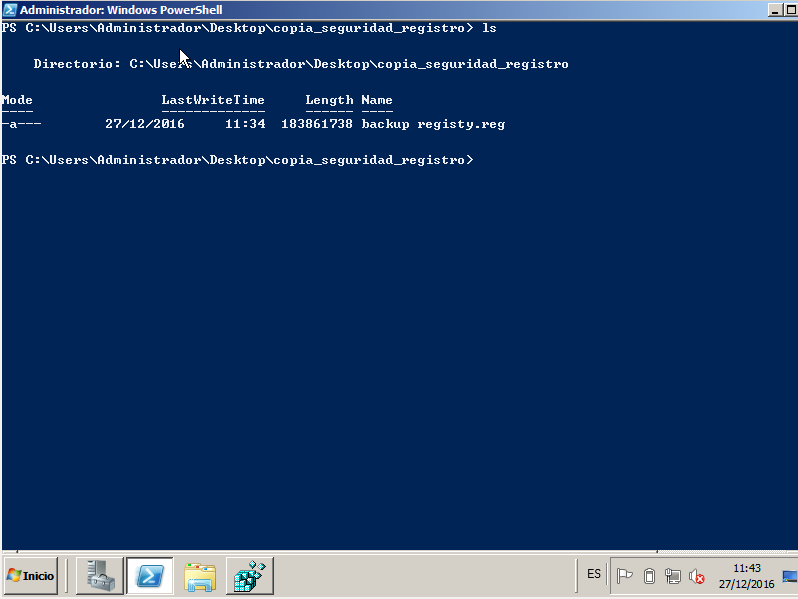
\includegraphics[scale=0.5]{ejercicio3-5.png} 
				\label{figura17} 
				\caption{Imagen 2: Resultados de ab para CentOS}
			\end{figure}
			
			\begin{figure}[H] 
				\centering
				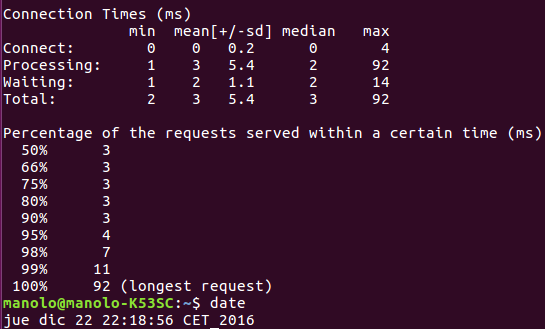
\includegraphics[scale=0.5]{ejercicio3-6.png} 
				\label{figura18} 
				\caption{Imagen 2: Resultados de ab para CentOS}
			\end{figure}
			
			Para CentOS podemos ver como el tiempo total del test es de 0.631 segundos. El tiempo media para cada petición es de 3.156 milisegundos. Dado que tenemos concurrencia 5, el tiempo medio de petición en concurrencia es de 3.156 ms / 5 = 0.631 ms.\\
			El total de bytes transferidos para Windows Server es de 5179000 bytes.
			
	\end{itemize}

	Los diferentes resultados muestran a simple vista como unas máquinas realizan en test en menor tiempo que otras, pero influyen diferentes variables para que eso ocurra. Por ejemplo la cantidad de bytes que tiene cada servidor es diferente y ha de transmitirse. También influyen otros aspectos como la red e incluso el tiempo de llamadas al sistema realizadas para llevar a cabo la ejecución de Apache Benchmark. Vemos como por ejemplo Ubuntu Server tardó en atender el 100\% de las peticiones 25 ms, mientras que Windows Server tardó 7 ms en atender el 100\% y mucho más CentOS, con 92 ms para atender el 100\% (de 99\% a 100\% CentOS tardó 92ms-11ms=81ms, una brutalidad). \\
	
	A primera vista podemos ver como Windows Server ha tardado 0.357 segundos en realizar el test, seguido de cerca por Ubuntu Server con 0.41 segundos y finalmente CentOS con 0.631 segundos.
	
	Mirando un poco más, vemos que la cantidad de bytes transferidos varían para cada uno. Tenemos a Ubuntu Server con 11783000 bytes, Windows Server con 931000 bytes y CentOS con 5179000 bytes. Eso se debe a que cada servidor tiene una página web predeterminada distinta y por tanto los bytes varían.\\
	Comparando la productividad de cada uno (Kbytes recibidos por segundo):
	\begin{itemize}
		\item Ubuntu Server: 28056.69 Kbytes / s
		\item Windows Server: 2543.35 Kbytes / s
		\item CentOS: 8013.2 bytes / ms
	\end{itemize}
	
	Según la productividad, el mejor es Ubuntu Server, seguido de CentOS y finalmente Windows Server .\\
	
	Hemos visto como la productividad de Ubuntu Server es la mejor, sin embargo Windows Server realiza el test en un tiempo menor. Esto se debe a que la cantidad de bytes que recibe Ubuntu Server es mucho mayor. Basándonos en estas características la mejor opción podría ser Ubuntu Server con Apache.\\
	
	Como conclusión final, es necesario decir que existen numerosas características a analizar de un servidor (muchas más de las analizadas) para determinar y concluir que sistema sería el mejor o adecuado para el uso que queramos darle. 
	
	%	Cuestión 4
	%-----------------------------------------------
	\section{Instale y siga el tutorial en http://jmeter.apache.org/usermanual/build-web-test-plan.html realizando capturas de pantalla y comentándolas. En vez de usar la web de jmeter, haga el experimento usando sus máquinas virtuales ¿coincide con los resultados de ab?}
	
	Vamos a ir por pasos para usar Jmeter, siguiendo como guía su página oficial\cite{ejercicio4-1}:
	\begin{itemize}
		\item Paso 1: Instalación de Jmeter por el gestor de paquetes:
			\begin{figure}[H] 
				\centering
				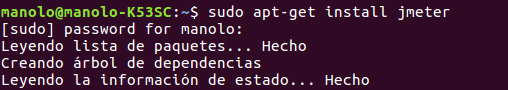
\includegraphics[scale=0.5]{ejercicio4-1.png} 
				\label{figura19} 
				\caption{Instalación de Jmeter}
			\end{figure}
		\item Paso 2: Ejecutamos el programa poniendo su nombre en el terminal y se nos abrirá:
			\begin{figure}[H] 
				\centering
				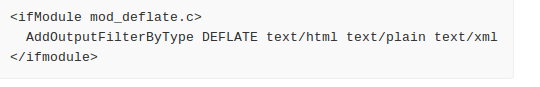
\includegraphics[scale=0.35]{ejercicio4-2.png} 
				\label{figura20} 
				\caption{Abrir Jmeter}
			\end{figure}
		\item Paso 3: Añadimos un Thread Group, que sirve para decirle a Jmeter el número de usuarios a simular, la frecuencia con la que los usuarios envían peticiones y cuantas peticiones deberían enviar. Para añadir, nos vamos al menú, pulsamos en "Editar", seleccionamos "Añadir", escogemos "Hilos (Usuarios)" y finalmente "Grupo de hilos". Nos deberá aparecer lo siguiente:
			\begin{figure}[H] 
				\centering
				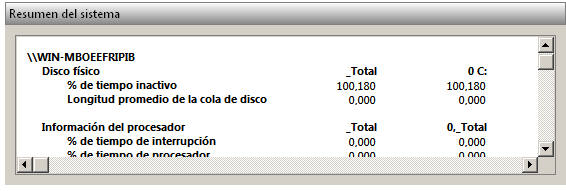
\includegraphics[scale=0.35]{ejercicio4-3.png} 
				\label{figura21} 
				\caption{Crear Grupo de hilos en Jmeter}
			\end{figure}
		\item Paso 4: Configuramos el grupo de hilos estableciendo "números de hilos" a 5 (serían los usuarios) y el número de veces que se va a repetir la prueba poniendo 100 en "Contador del bucle".
			\begin{figure}[H] 
				\centering
				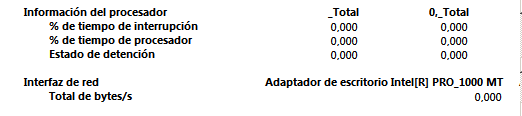
\includegraphics[scale=0.35]{ejercicio4-4.png} 
				\label{figura22} 
				\caption{Configurar Grupo de hilos en Jmeter}
			\end{figure}
		\item Paso 5: Añadir las propiedades por defecto para peticiones HTTP. Una vez que tenemos los usuarios, se definen las tareas que realizarán. Vamos a configurar las peticiones HTTP por defecto.\\
		Para añadir peticiones HTTP por defecto hacemos click derecho sobre "Grupo de hilos" y hacemos "Añadir" >  "Elemento de configuración" > "Valores por defecto para petición HTTP". Nos deberá aparecer lo siguiente:
			\begin{figure}[H] 
				\centering
				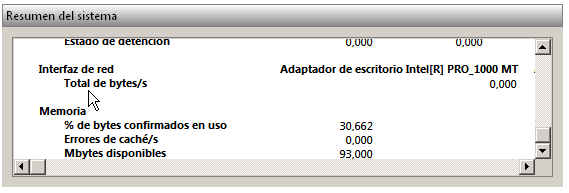
\includegraphics[scale=0.35]{ejercicio4-5.png} 
				\label{figura23} 
				\caption{Añadir valores por defecto para petición HTTP al Grupo de hilos}
			\end{figure}
		\item Paso 6: Establecemos el nombre del servidor o IP (será la de las máquinas virtuales) en el campo  "Nombre del Servidor o IP" dentro de los Valores por Defecto para Petición HTTP. Se modificará más adelante conforme se prueben las diferentes máquinas.
		\item Paso 7: Añadir soporte a cookies. Vamos a activarlas, para ello click derecho sobre "Grupo de hilos" y hacemos "Añadir" >  "Elemento de configuración" > "Gestor de cookies HTTP". Nos deberá quedar así:
			\begin{figure}[H] 
				\centering
				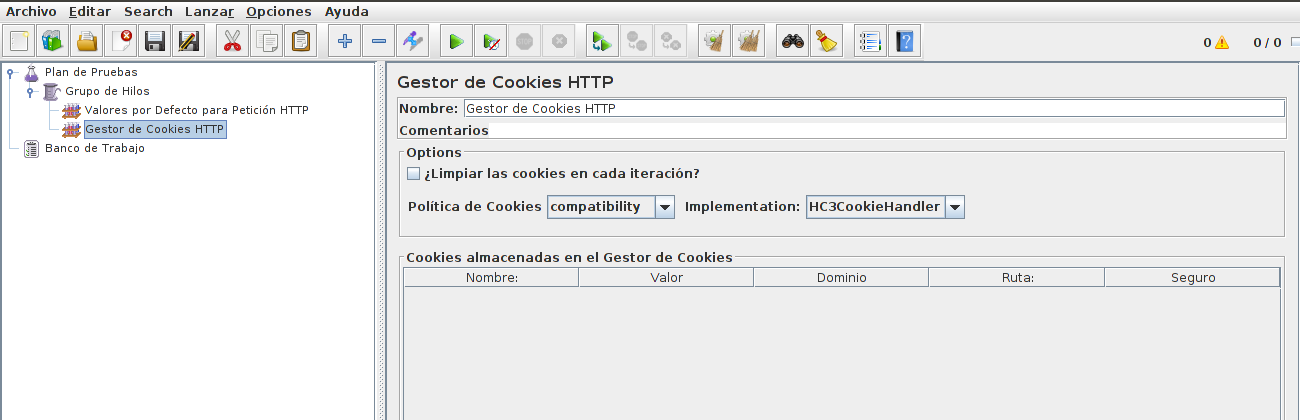
\includegraphics[scale=0.35]{ejercicio4-6.png} 
				\label{figura24} 
				\caption{Añadir gestor de cookies HTTP al Grupo de hilos}
			\end{figure}
		\item Paso 8: Añadir petición HTTP. Para ello click derecho sobre "Grupo de hilos" y "Añadir" > "Muestreador" > "Petición HTTP". Nos deberá quedar de esta forma:
			\begin{figure}[H] 
				\centering
				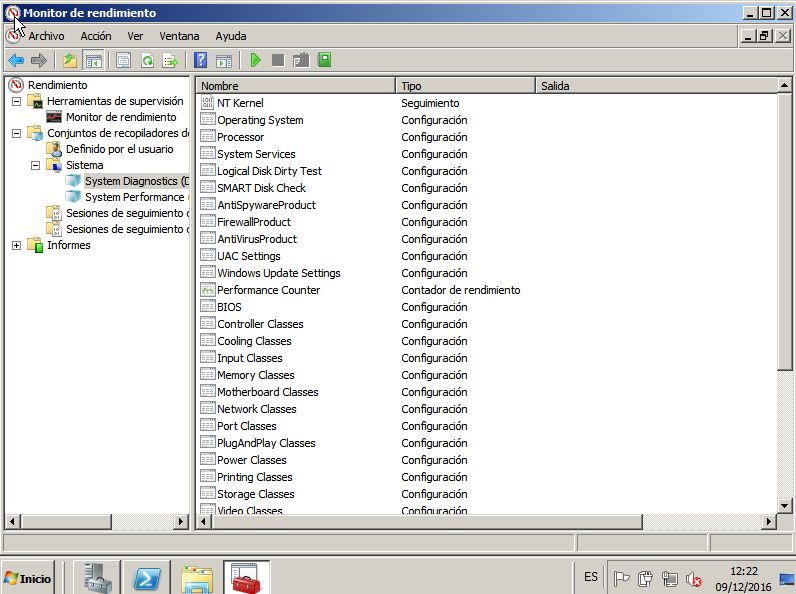
\includegraphics[scale=0.35]{ejercicio4-7.png} 
				\label{figura25} 
				\caption{Añadir petición HTTP al Grupo de hilos}
			\end{figure}
		\item Paso 9: Añadir un oyente para que almacene los datos de la prueba. Se encarga de almacenar los resultados de las peticiones HTTP en un archivo y los presenta de forma gráfica. Para añadirlo, click derecho sobre "Grupo de hilos" y "Añadir" > "Receptor" > "Gráfico de Resultados". Veremos lo siguiente:
			\begin{figure}[H] 
				\centering
				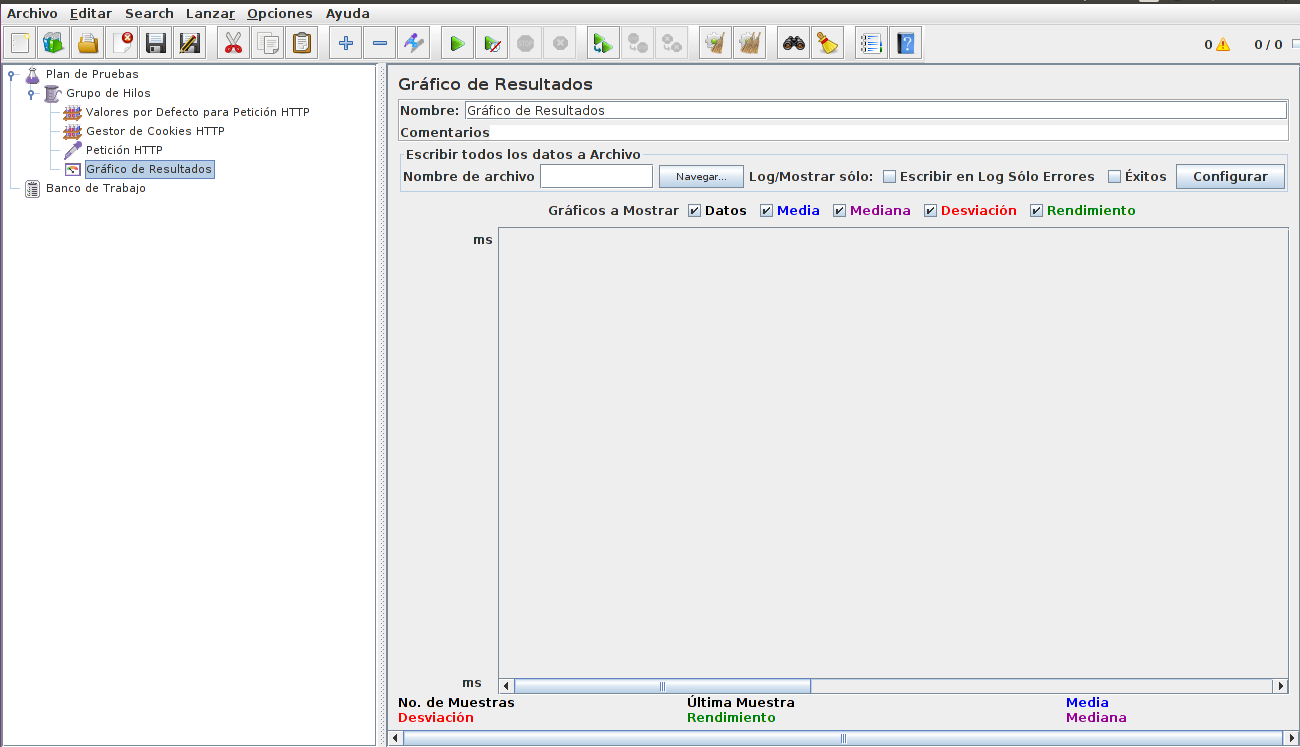
\includegraphics[scale=0.35]{ejercicio4-8.png} 
				\label{figura26} 
				\caption{Añadir gráfico de resultados al Grupo de hilos}
			\end{figure}
	\end{itemize}
	
	Probamos con phyadmin desde la máquina de Ubuntu Server, para ello tenemos que hemos configurado lo siguiente:
	\begin{itemize}
		\item Ponemos a 1000 el bucle y con 5 usuarios (esto serán 5000 muestras).
			\begin{figure}[H] 
				\centering
				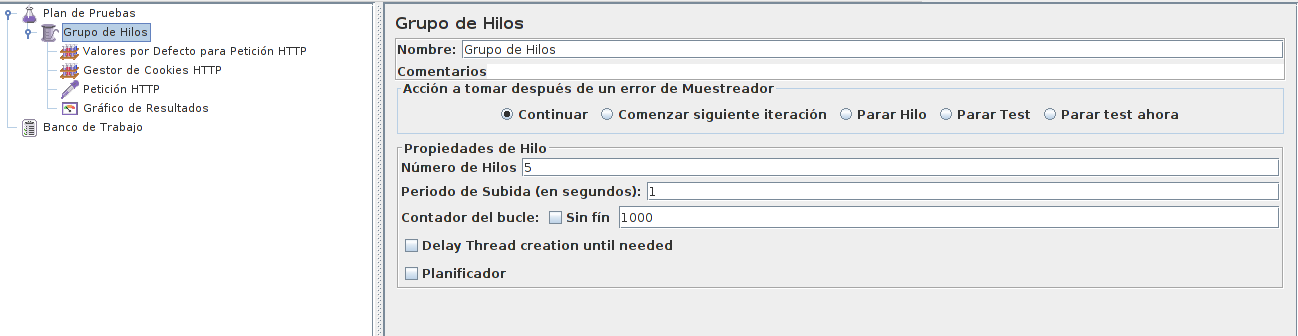
\includegraphics[scale=0.35]{ejercicio4-9.png} 
				\label{figura27} 
				\caption{Jmeter con 5000 muestras}
			\end{figure}
		\item Ponemos la url de phpmyadmin en "Valores por defecto para petición HTTP":
			\begin{figure}[H] 
				\centering
				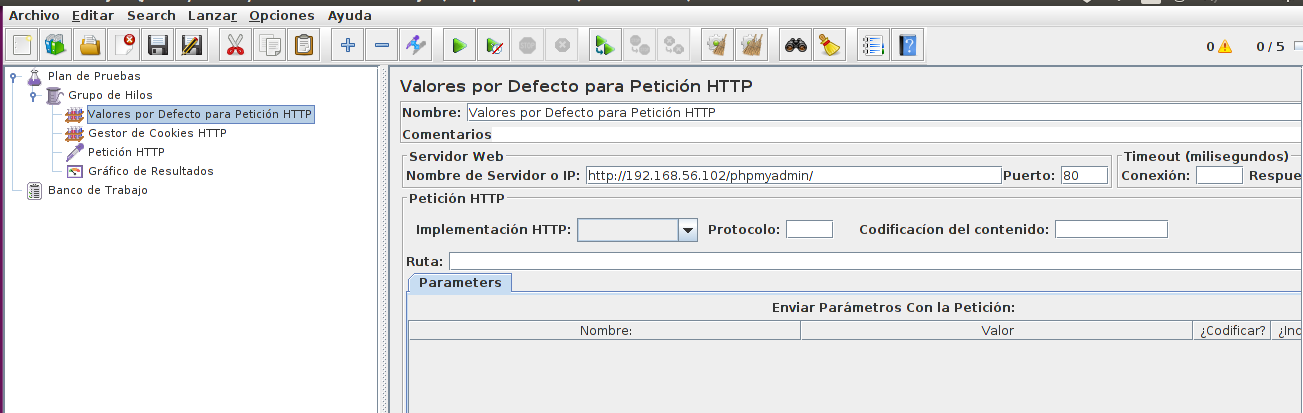
\includegraphics[scale=0.35]{ejercicio4-10.png} 
				\label{figura28} 
				\caption{Configurar valores por defecto para peticion HTTP en Jmeter para phpmyadmin}
			\end{figure}
		\item Configuramos la petición HTTP y establecemos valores que se pasan por ella, que serán el usuario y contraseña para phpymyadmin:
			\begin{figure}[H] 
				\centering
				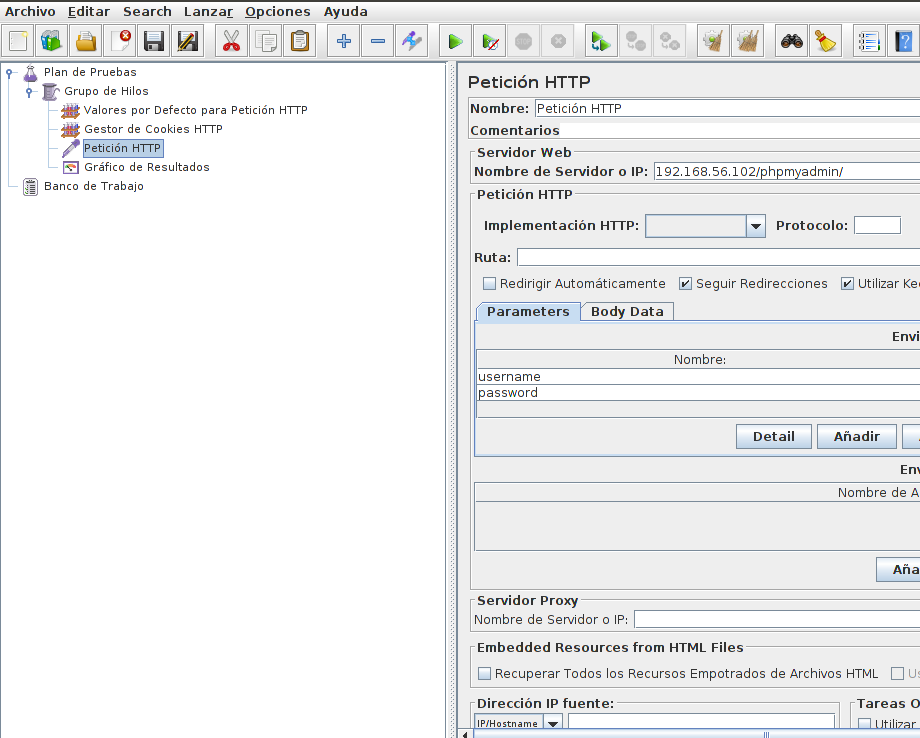
\includegraphics[scale=0.35]{ejercicio4-11.png} 
				\label{figura29} 
				\caption{Configurar la petición HTTP en Jmeter para phpmyadmin}
			\end{figure}
		\item Lanzamos el test y comprobamos el gráfico:
			\begin{figure}[H] 
				\centering
				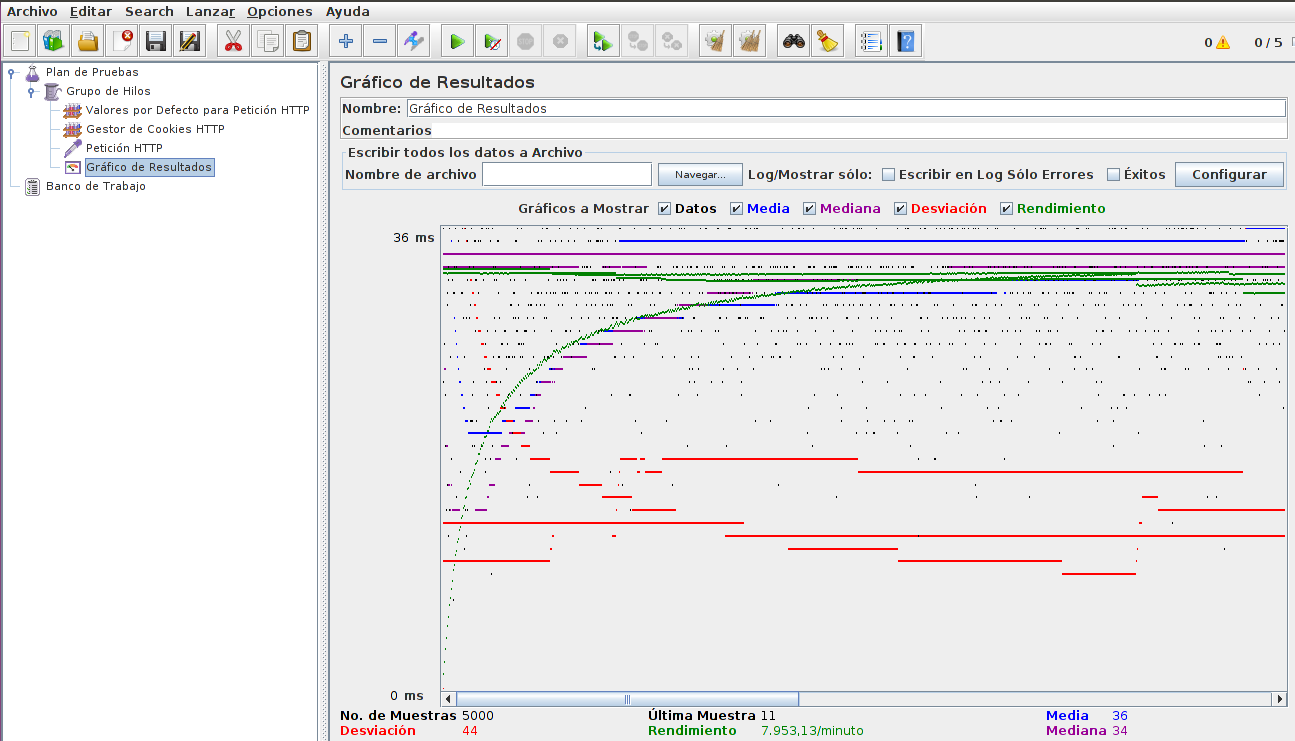
\includegraphics[scale=0.35]{ejercicio4-12.png} 
				\label{figura30} 
				\caption{Gráfico generado tras en test en Jmeter para phpmyadmin}
			\end{figure}
		\item Lanzamos con ab el mismo test, con 5000 muestras y 5 hebras.
			\begin{figure}[H] 
				\centering
				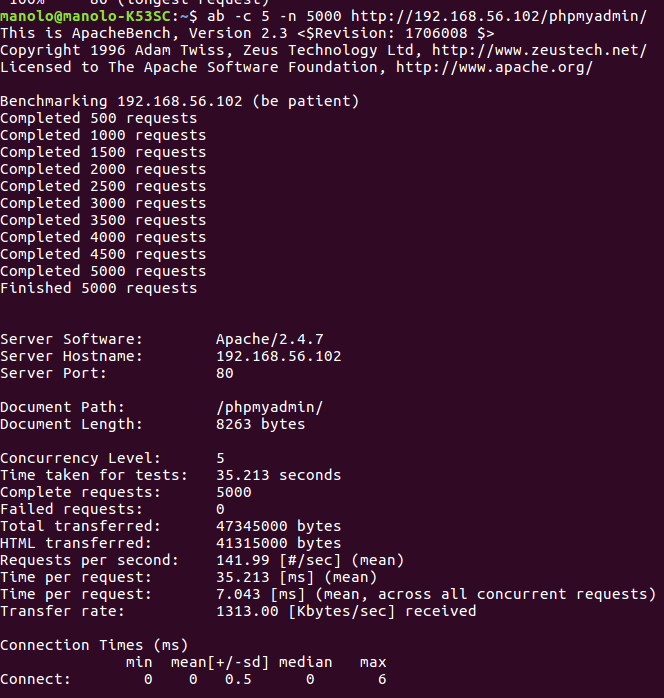
\includegraphics[scale=0.35]{ejercicio4-13.png} 
				\label{figura31} 
				\caption{Imagen 1:Mismo test con ab que en Jmeter para phpmyadmin}
			\end{figure}
			\begin{figure}[H] 
				\centering
				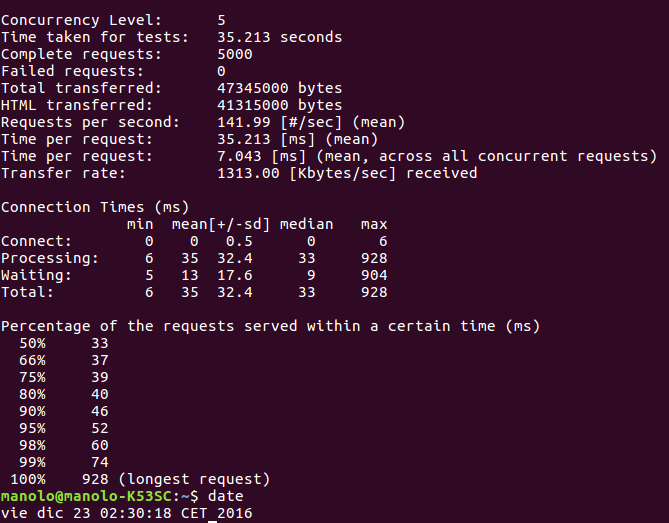
\includegraphics[scale=0.35]{ejercicio4-14.png} 
				\label{figura32} 
				\caption{Imagen 2:Mismo test con ab que en Jmeter para phpmyadmin}
			\end{figure}
	\end{itemize}
	
	En la gráfica nos sale media 36, mediana 34 y desviación 44 para 5000 muestras. Con ab sale una media de 35 y una mediana de 33 con una desviación de 32.4. Los resultados son muy parecidos por lo que se puede decir que casi prácticamente coinciden.
	%----------------------------------------------------------------------------------------
	%	Cuestión 5
	%----------------------------------------------------------------------------------------
	
	\section{Programe un benchmark usando el lenguaje que desee. El benchmark debe incluir:
		1) Objetivo del benchmark.
		2) Métricas (unidades, variables, puntuaciones, etc.).
		3) Instrucciones para su uso.
		4) Ejemplo de uso analizando los resultados.}
	
	\subsection{1) Objetivo del benchmark}
	
	El objetivo del benchmark consiste en mandar información por un socket para ver cual es la velocidad máxima de transferencia utilizando para ello diferentes tamaños de paquetes. Un socket es la transferencia básica de información en Internet, es un punto final de un enlace de comunicación bidireccional entre dos programas que se ejecutan en la red. Está enlazado a un número de puerto para que la capa TCP pueda identificar la aplicación a la que se destinan los datos\cite{ejercicio5-1,ejercicio5-2,ejercicio5-3,ejercicio5-4,ejercicio5-5,ejercicio5-6,ejercicio5-7,ejercicio5-8,ejercicio5-9,ejercicio5-10,ejercicio5-11,ejercicio5-12,ejercicio5-13}.
	
	\subsection{2) Métricas (unidades, variables, puntuaciones, etc.).}
	
	Para la velocidad son MB/s y tamaño de los paquetes en bytes.
	
	\subsection{3) Instrucciones para su uso.}
	
	Para su uso basta con compilarlo con la orden gcc -o bench bench.c y posteriormente ejecutarlo con ./benchmark.
	
	\subsection{4) Ejemplo de uso analizando los resultados.}
	
	
	Se crean un proceso padre y otro hijo los cuales crean una vía de comunicación para enviarse y recibir información usando para ello el localhost (127.0.0.1). Para diferentes tamaños de paquete va midiendo la velocidad de transferencia y muestra la velocidad más óptima y el tamaño de paquete que consigue dicha velocidad.\\
	
	El código usado para el benchmark es el siguiente:
	
	\begin{figure}[H] 
		\centering
		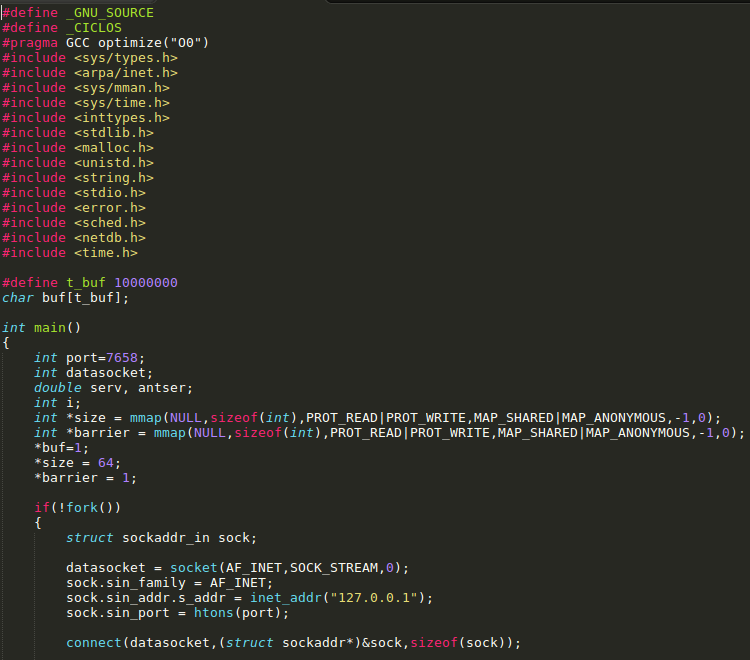
\includegraphics[scale=0.35]{ejercicio5-1.png} 
		\label{figura33} 
		\caption{Imagen 1: Código del benchmark}
	\end{figure}
	
	\begin{figure}[H] 
		\centering
		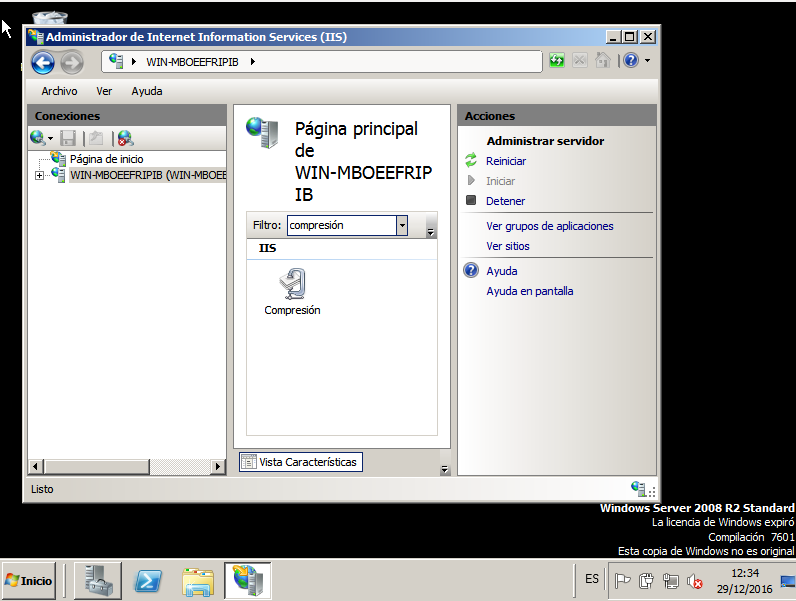
\includegraphics[scale=0.35]{ejercicio5-2.png} 
		\label{figura34} 
		\caption{Imagen 2:Código del benchmark}
	\end{figure}
	
	\begin{figure}[H] 
		\centering
		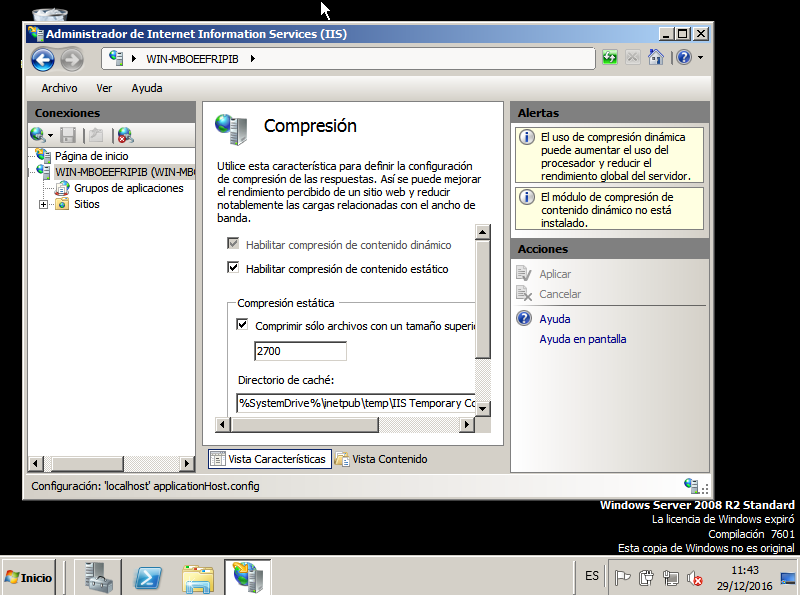
\includegraphics[scale=0.35]{ejercicio5-3.png} 
		\label{figura35} 
		\caption{Imagen 3:Código del benchmark}
	\end{figure}
	
	Aquí vemos un ejemplo de ejecución:
	
	\begin{figure}[H] 
		\centering
		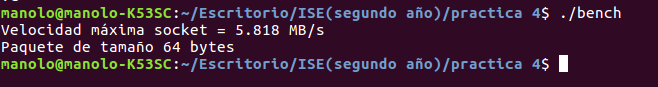
\includegraphics[scale=0.35]{ejercicio5-4.png} 
		\label{figura36} 
		\caption{Ejecución del benchmark}
	\end{figure}
	
	Podemos ver como para un socket el tamaño adecuado para la máxima velocidad es 64 bytes, no más ni menos ya que para tamaños superiores e inferiores no irá a la velocidad indicada por este, la cual es de 5.8188 MB/s.
	
	%----------------------------------------------------------------------------------------
	%	Cuestión opcional 1
	%----------------------------------------------------------------------------------------
	\section{Opcional 1: ¿Qué es Scala? Instale Gatling y pruebe los escenarios por defecto.}
	



	

%------------------------------------------------

\bibliography{citas} %archivo citas.bib que contiene las entradas 
\bibliographystyle{plain} % hay varias formas de citar

\end{document}
